\section{Design Procedure}\label{sec:methods}
\begin{figure}[!h]
    \centering
        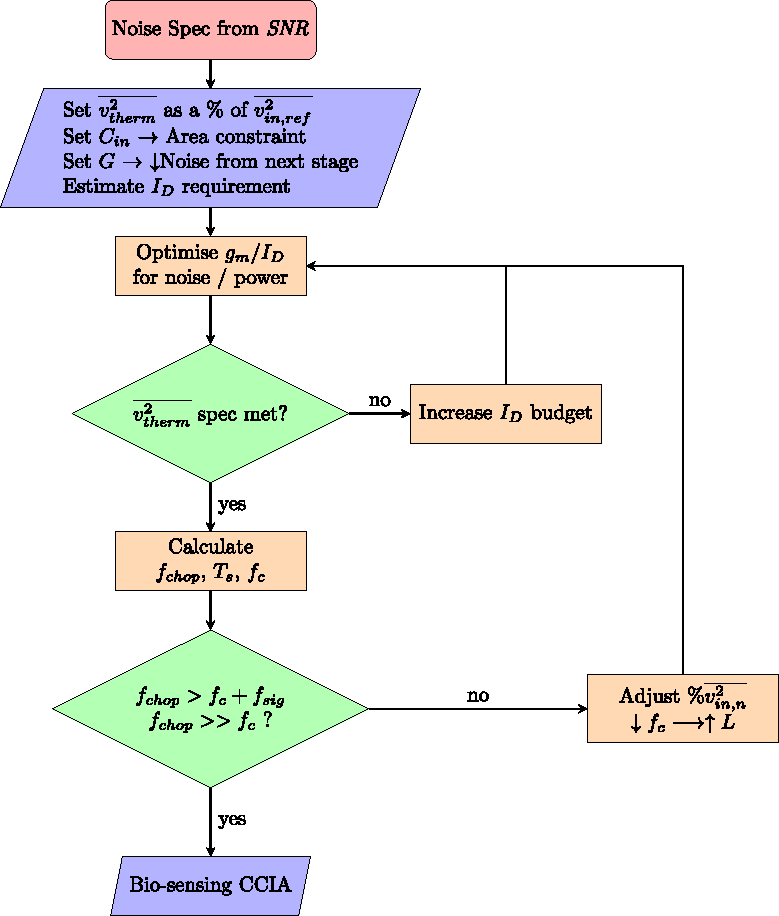
\includegraphics[width=0.8\linewidth]{img/DesignFlow.pdf}
    \caption{Design flow}
    \label{fig:design flow}
\end{figure}

This paper employs a systematic methodology (see \Cref{fig:design flow}) for designing an optimised CCIA, with a focus on achieving an area-aware design with optimal noise and power performance. A repeatable design flow is recorded in a Python Jupyter Notebook\cite{CCIA_GMID}, using PyGMID\cite{O_Donnell_PyGMID}. The optimisation procedure is as follows:
\subsection{Setting Initial Values}
The SNR, minimum signal amplitude ${V_{in}}$ and bandwidth requirements dictate a specification for the maximum input referred noise power spectral density $\overline{v_{in,ref}^2}$ . Referring to \cref{eq:system_noise} in this design example $\overline{v_{n,sensor}^2}=0$. Assuming that $\overline{v_{f_c}^2}$ contributions can be reduced through chopping \cite{Ha-8410446}, $\overline{v_{therm}^2}$ is apportioned a percentage of $\overline{v_{in,ref}^2}$. An initial $C_{in}$ is determined based on a fraction ($\kappa$) of the desired CCIA area (A). $C_{in}$ is calculated as: $C_{in}= \text{Capacitance Density} \times \kappa A$. In this example, $C_{in}=\SI{10}{\pico\farad}$.

The closed loop gain ($G$) is chosen large enough so that noise contributions from successive stages are insignificant. In this example, $G=\SI{20}{\frac{\volt}{\volt}}$. By re-arranging \cref{eq:vinamp} and with an initial estimate of \gmID, we can approximate the $I_{D}$ required to achieve the desired CCIA IRN. 

\subsection{Optimise $g_m/I_D$ for Noise, Power and Area}
\begin{figure} [!htbp]
    \centering
    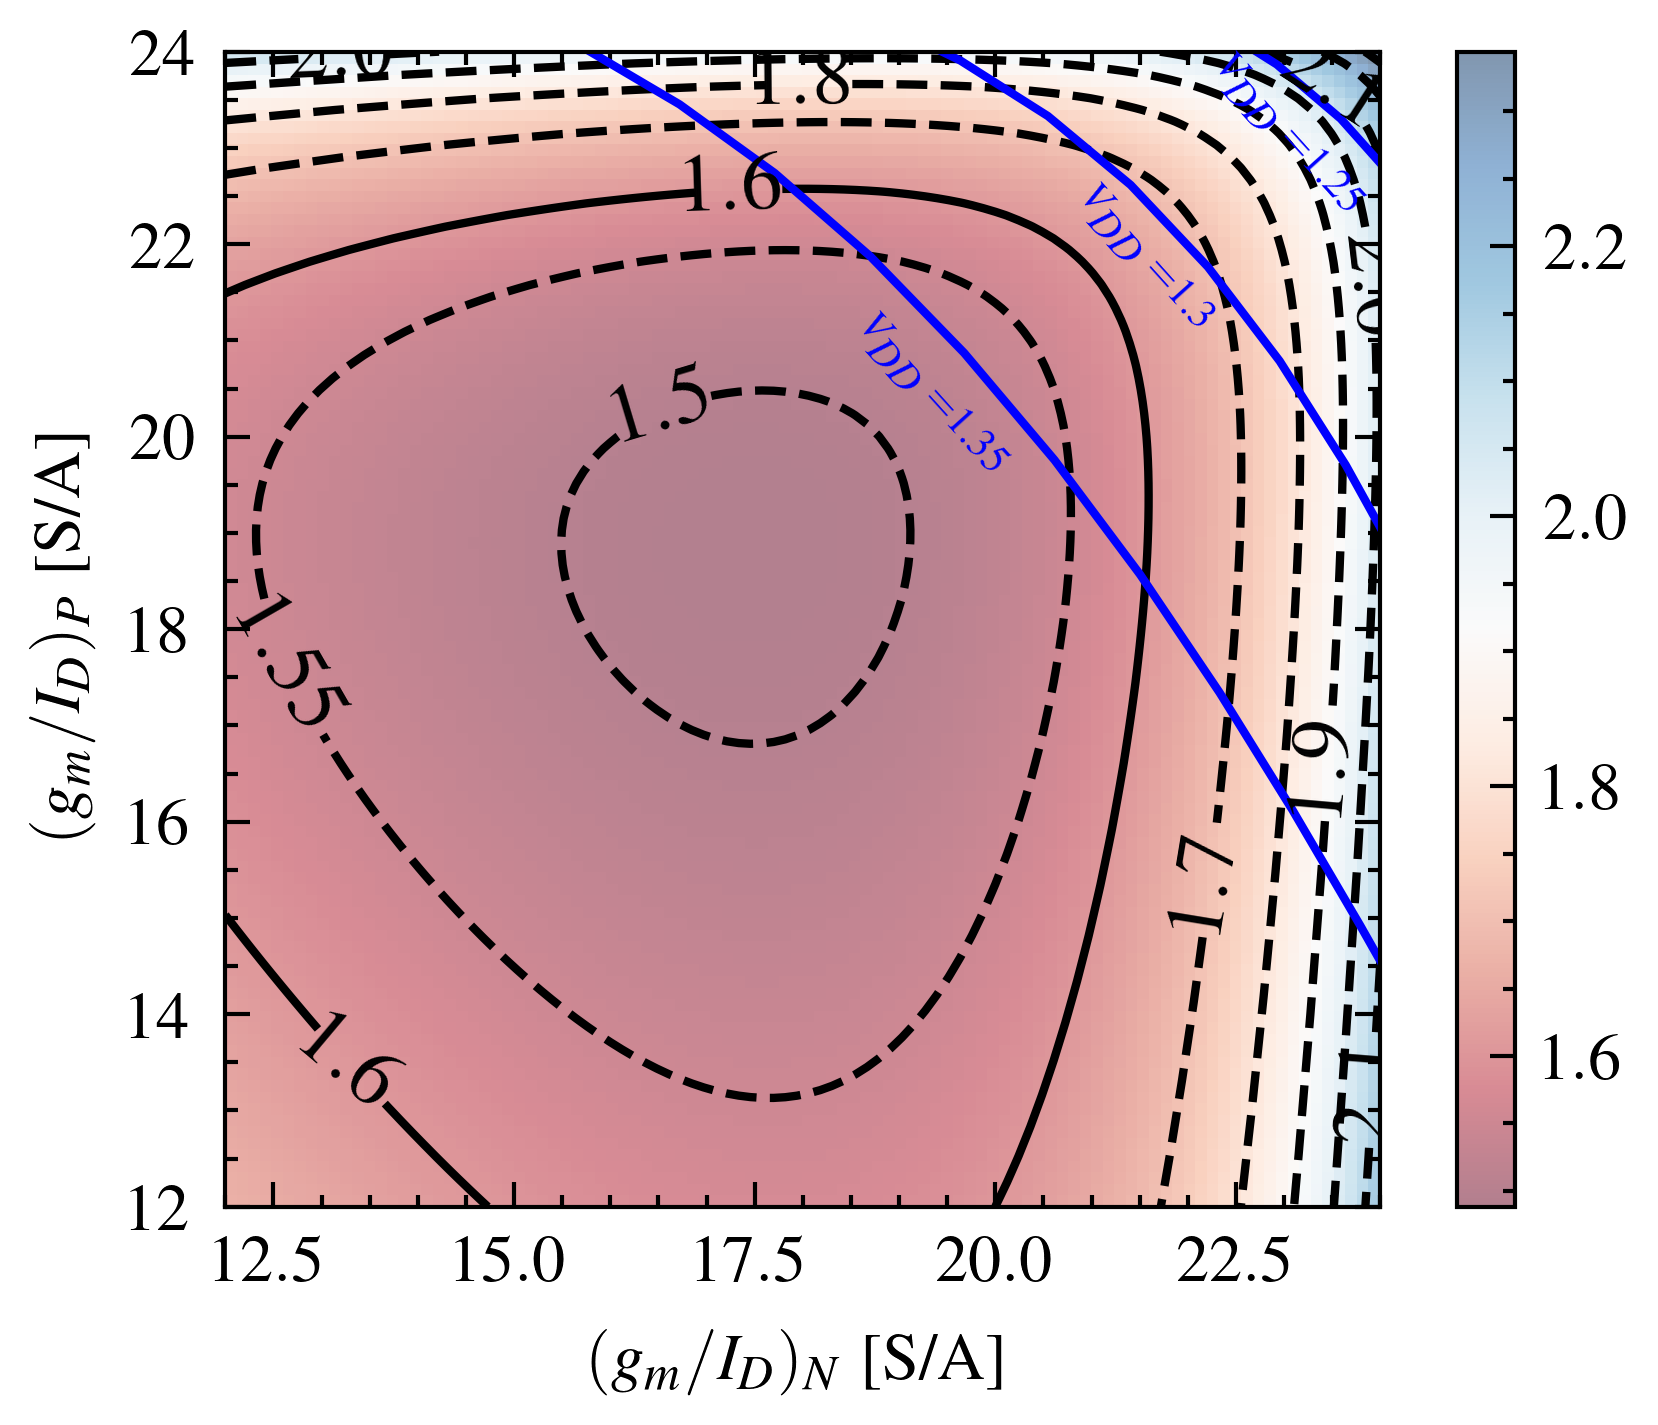
\includegraphics[ width = 0.7\columnwidth]{img/GM_ID_IRN.png} 
    \caption{ IRN ($\si{\nano\volt\per\sqrt{\hertz}}$) as a function of $(g_m/I_D)_N$ and $(g_m/I_D)_P$. $C_{in}=\SI{10}{\pico\farad}$ and $G=20$.}
    \label{fig:GM_ID_VS_IRN}
\end{figure}

The next step involves optimising \gmID ratios of the differential pairs. \Cref{fig:GM_ID_VS_IRN} illustrates CCIA IRN using \cref{eq:system_noise}. It is assumed that increasing \gmID will improve the IRN. However, this increases $C_g$, with a subsequent increase in noise gain factor ($\eta$) and IRN. The shallow optimum for IRN is denoted by the solid black line for \gmID ratios of 15 to 20. Using the same bias for the PMOS and NMOS differential pair requires a supply voltage of $V_{DD} \geq V_{GS,M1} + V_{GS,M3} + 2V_{DS}$. The supply voltage requirement to satisfy this condition and achieve an optimal \gmID for the targeted IRN, is denoted by solid blue lines. The dual-loop CCIA (DL-CCIA) (see \cref{sec:implementation}), allows separate biasing for the PMOS and NMOS devices, removing the supply voltage constraint \cite{srivastava20243d}. This technique is useful when high $V_T$ thick oxide devices are utilised to minimise gate leakage. If the IRN specification is not met with the initial design values, $I_D$ is increased, and the \gmID optimisation process repeated (as shown in \cref{fig:design flow}).
 
In the next step, $f_{chop}$, $T_{settle}$ (see \cref{eq:Settle_time}), and $f_{c}$ are calculated. $f_{chop}$ should be greater than $f_{c}$ to ensure effective flicker noise suppression from the filter. \Cref{fig:flicker} shows $f_c$ versus \gmID for various ratios of NMOS to PMOS channel length. $f_c$ can be reduced by increasing \gmID. Additionally, it is observed that $f_c$ is more influenced by the NMOS device in the \SI{65}{\nano\metre} process. Thus, maintaining $L_N/L_P > 1$ helps achieve a lower $f_c$. $f_c$ reductions for $L_N/L_P > 1.4$ appear diminishing in comparison to the increased area cost. The reduction of $f_c$ with respect to \gmID leads to an increase in $C_g$ (see \Cref{fig:trade-off}), which in turn increases the noise gain $\eta$ and IRN. It can be seen from \Cref{fig:trade-off} that $g_m/I_D\approx 18$ is an optimal region that balances minimum IRN, $C_g$ and $f_c$ for the area-aware design presented in this work.  

\begin{figure}[!h]
        \centering
        \begin{subfigure}[c]{0.42\linewidth}
            \centering
            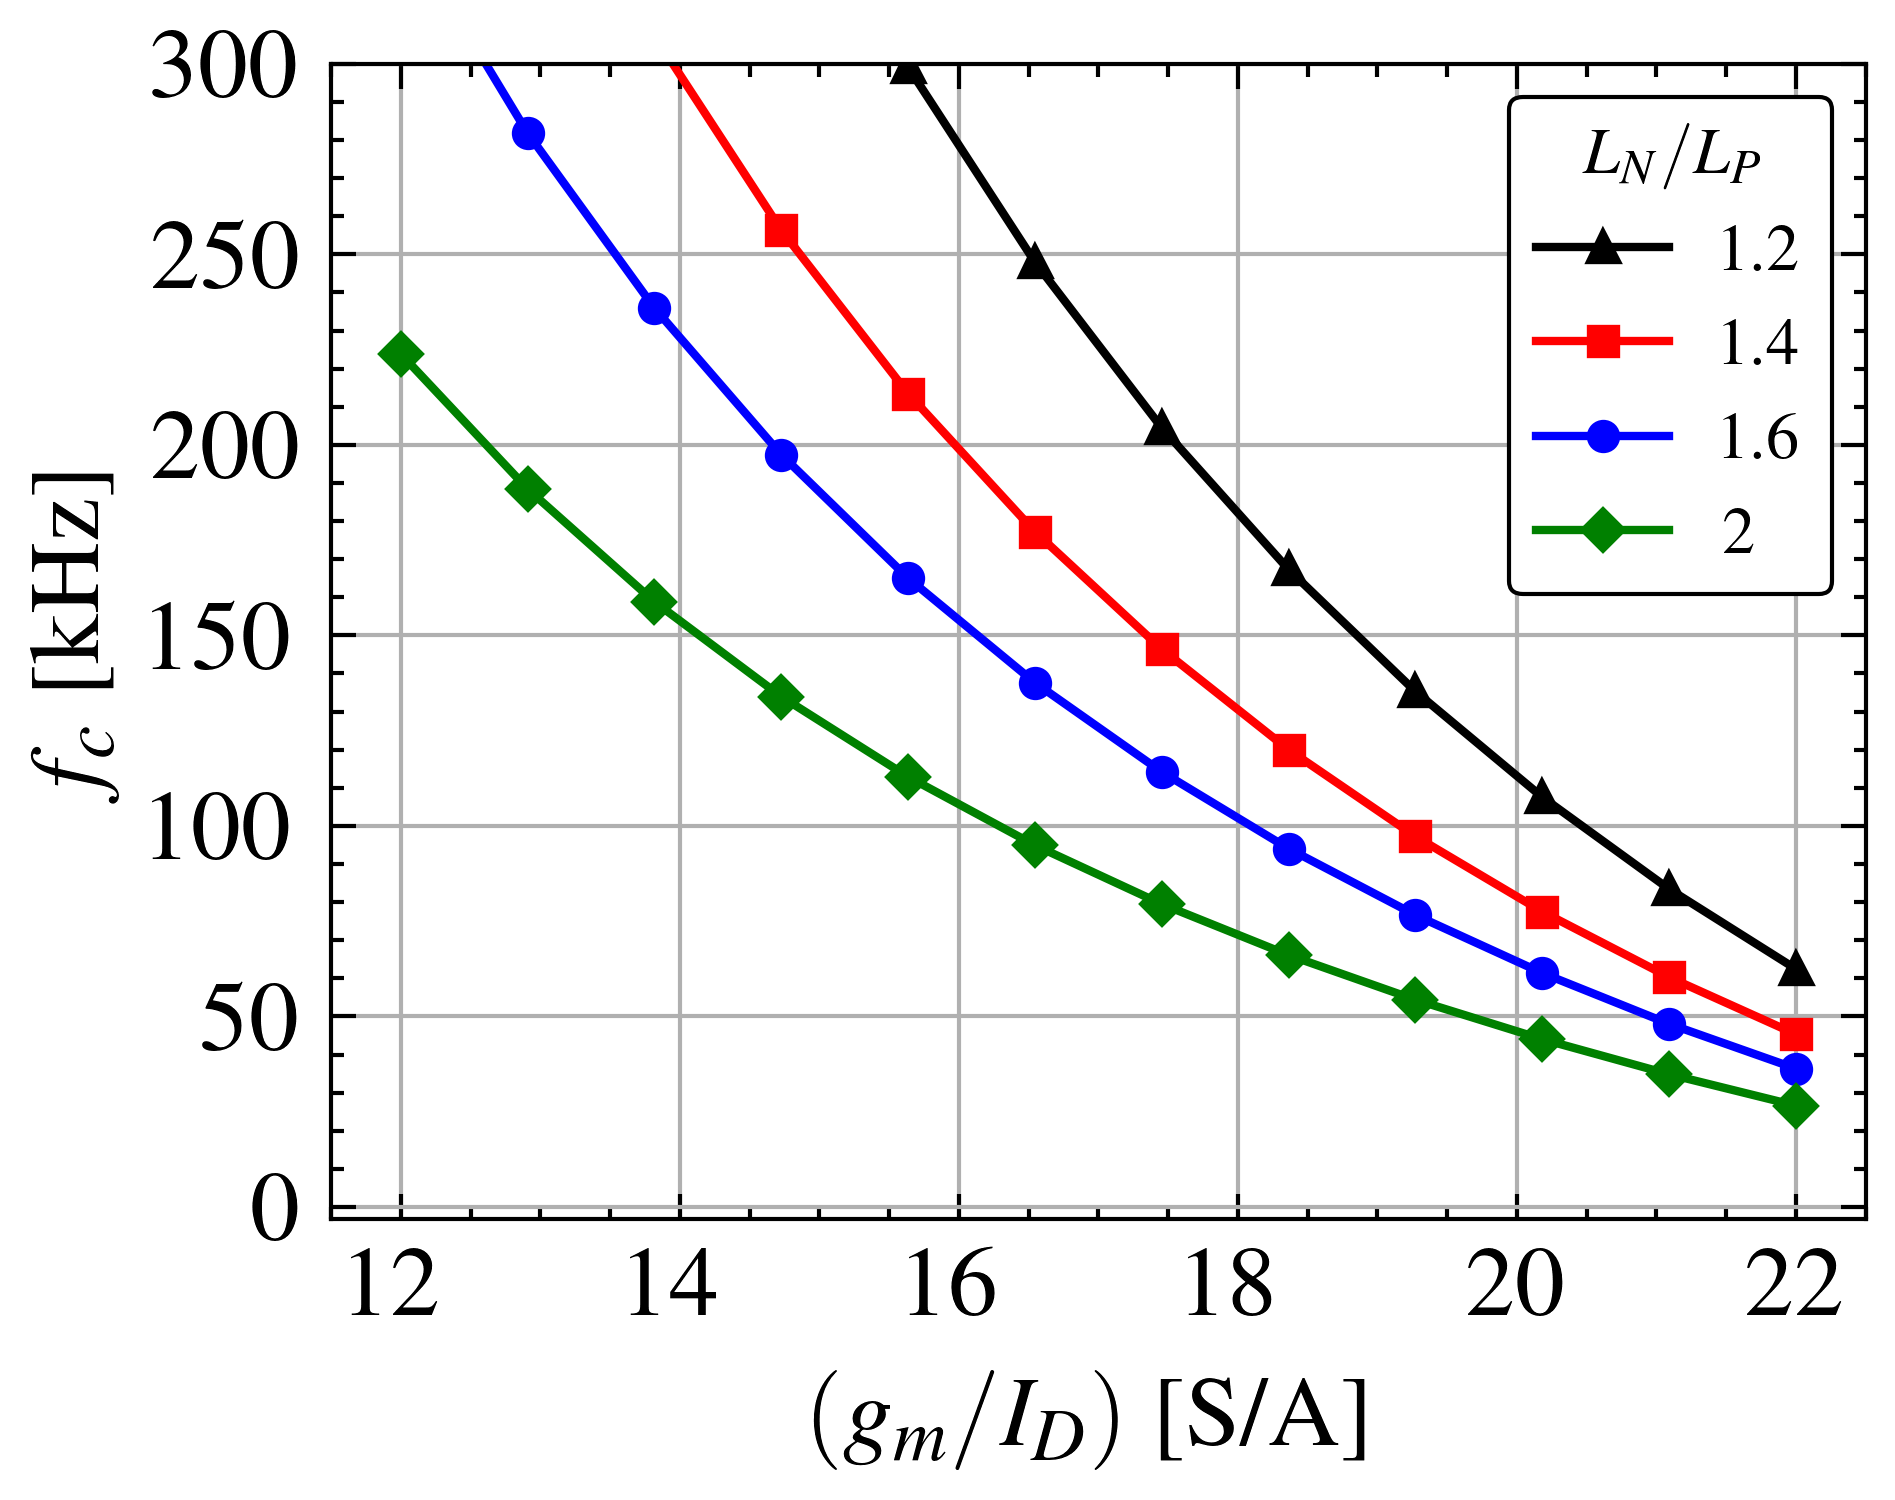
\includegraphics[width=\linewidth]{img/flicker.png}
            \caption[]%
            {{\small }}
            \label{fig:flicker}
        \end{subfigure}
        \hfill
        \begin{subfigure}[c]{0.53\linewidth}  
            \centering 
            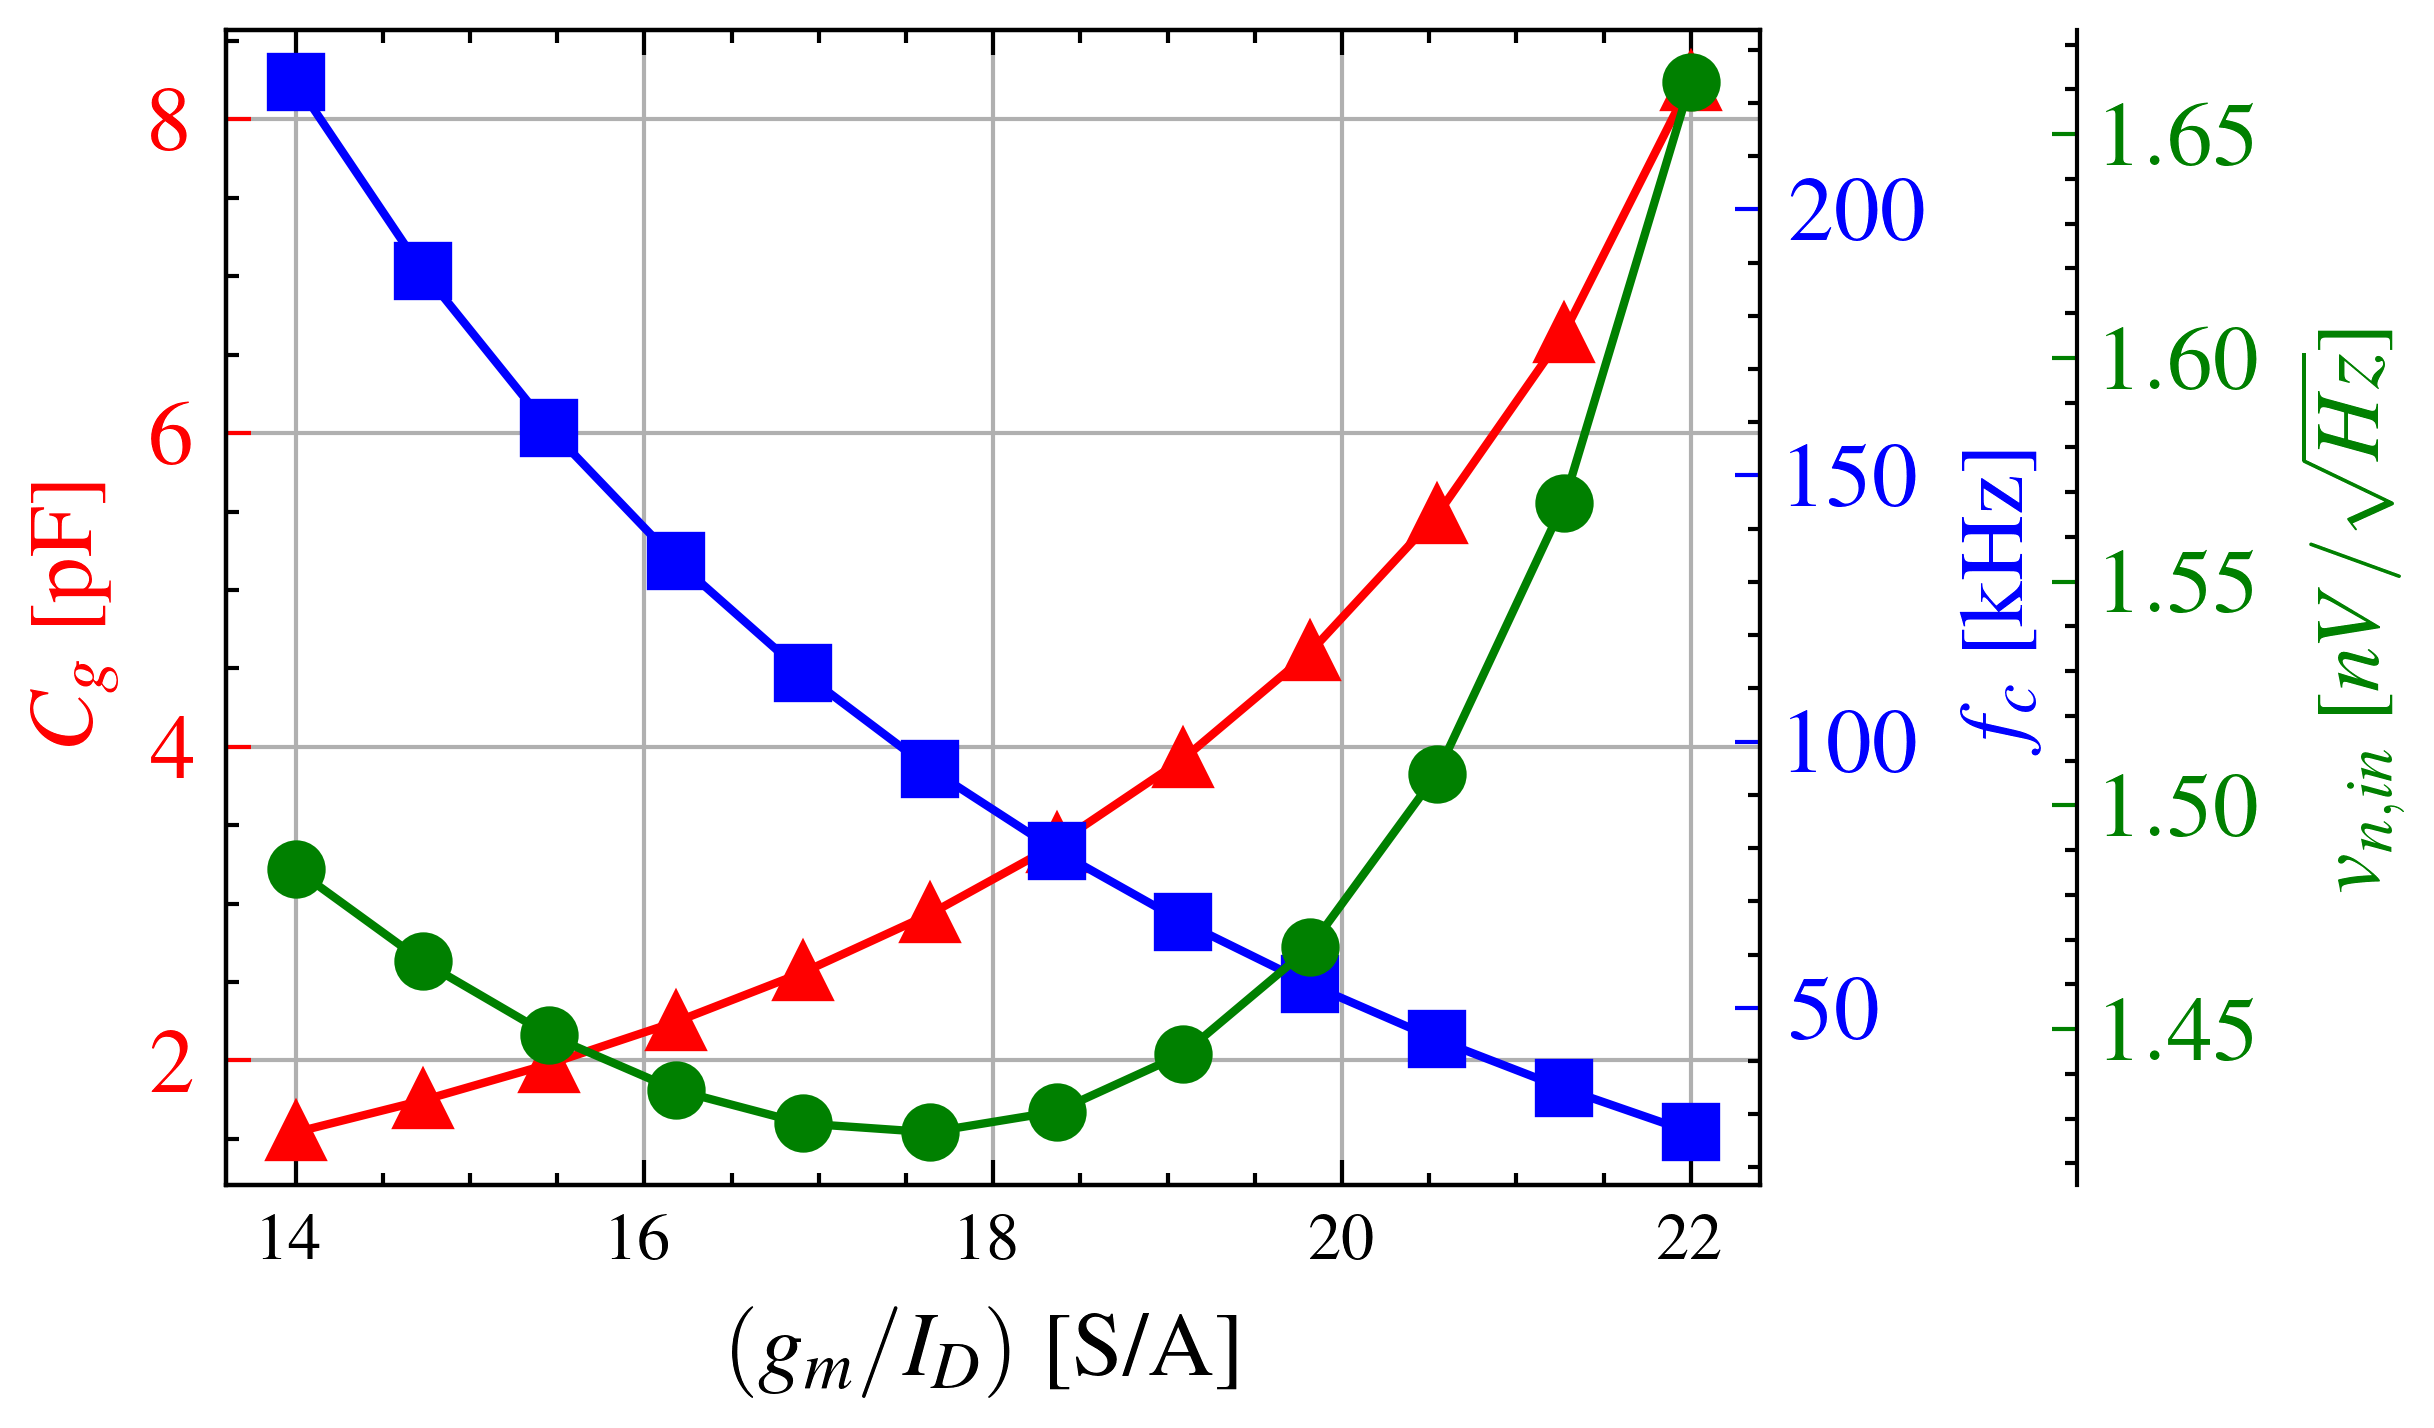
\includegraphics[width=\linewidth]{img/trade-off.png}
            \caption[]%
            {{\small }}
            \label{fig:trade-off}
        \end{subfigure}
        \caption[ Don't write caption here ]
        {\small (a) {$f_{c}$ vs. \gmID for different ratios of NMOS and PMOS lengths } (b) $f_{c}$, $C_{g}$ and IRN vs. \gmID for $L_N/L_P=1.4$} 
        \label{fig:flicker and trade off}
\end{figure}

\subsection{Iterations}
If frequency criteria are not met, further adjustments are required to refine the design. The percentage of $\overline{v_{in,ref}^2}$ allocated to $\overline{v_{therm}^2}$ can be increased and/or the device lengths could be increased to reduce $f_{c}$. This iterative refinement process, which involves recalculating IRN, \gmID, $C_{in}$, $f_{chop}$ and $f_c$ continues until all conditions are satisfied. This approach ensures convergence upon an area-aware design with optimal noise and power performance.

\begin{figure}[!h]
        \centering
        \begin{subfigure}[c]{0.49\linewidth}
            \centering
            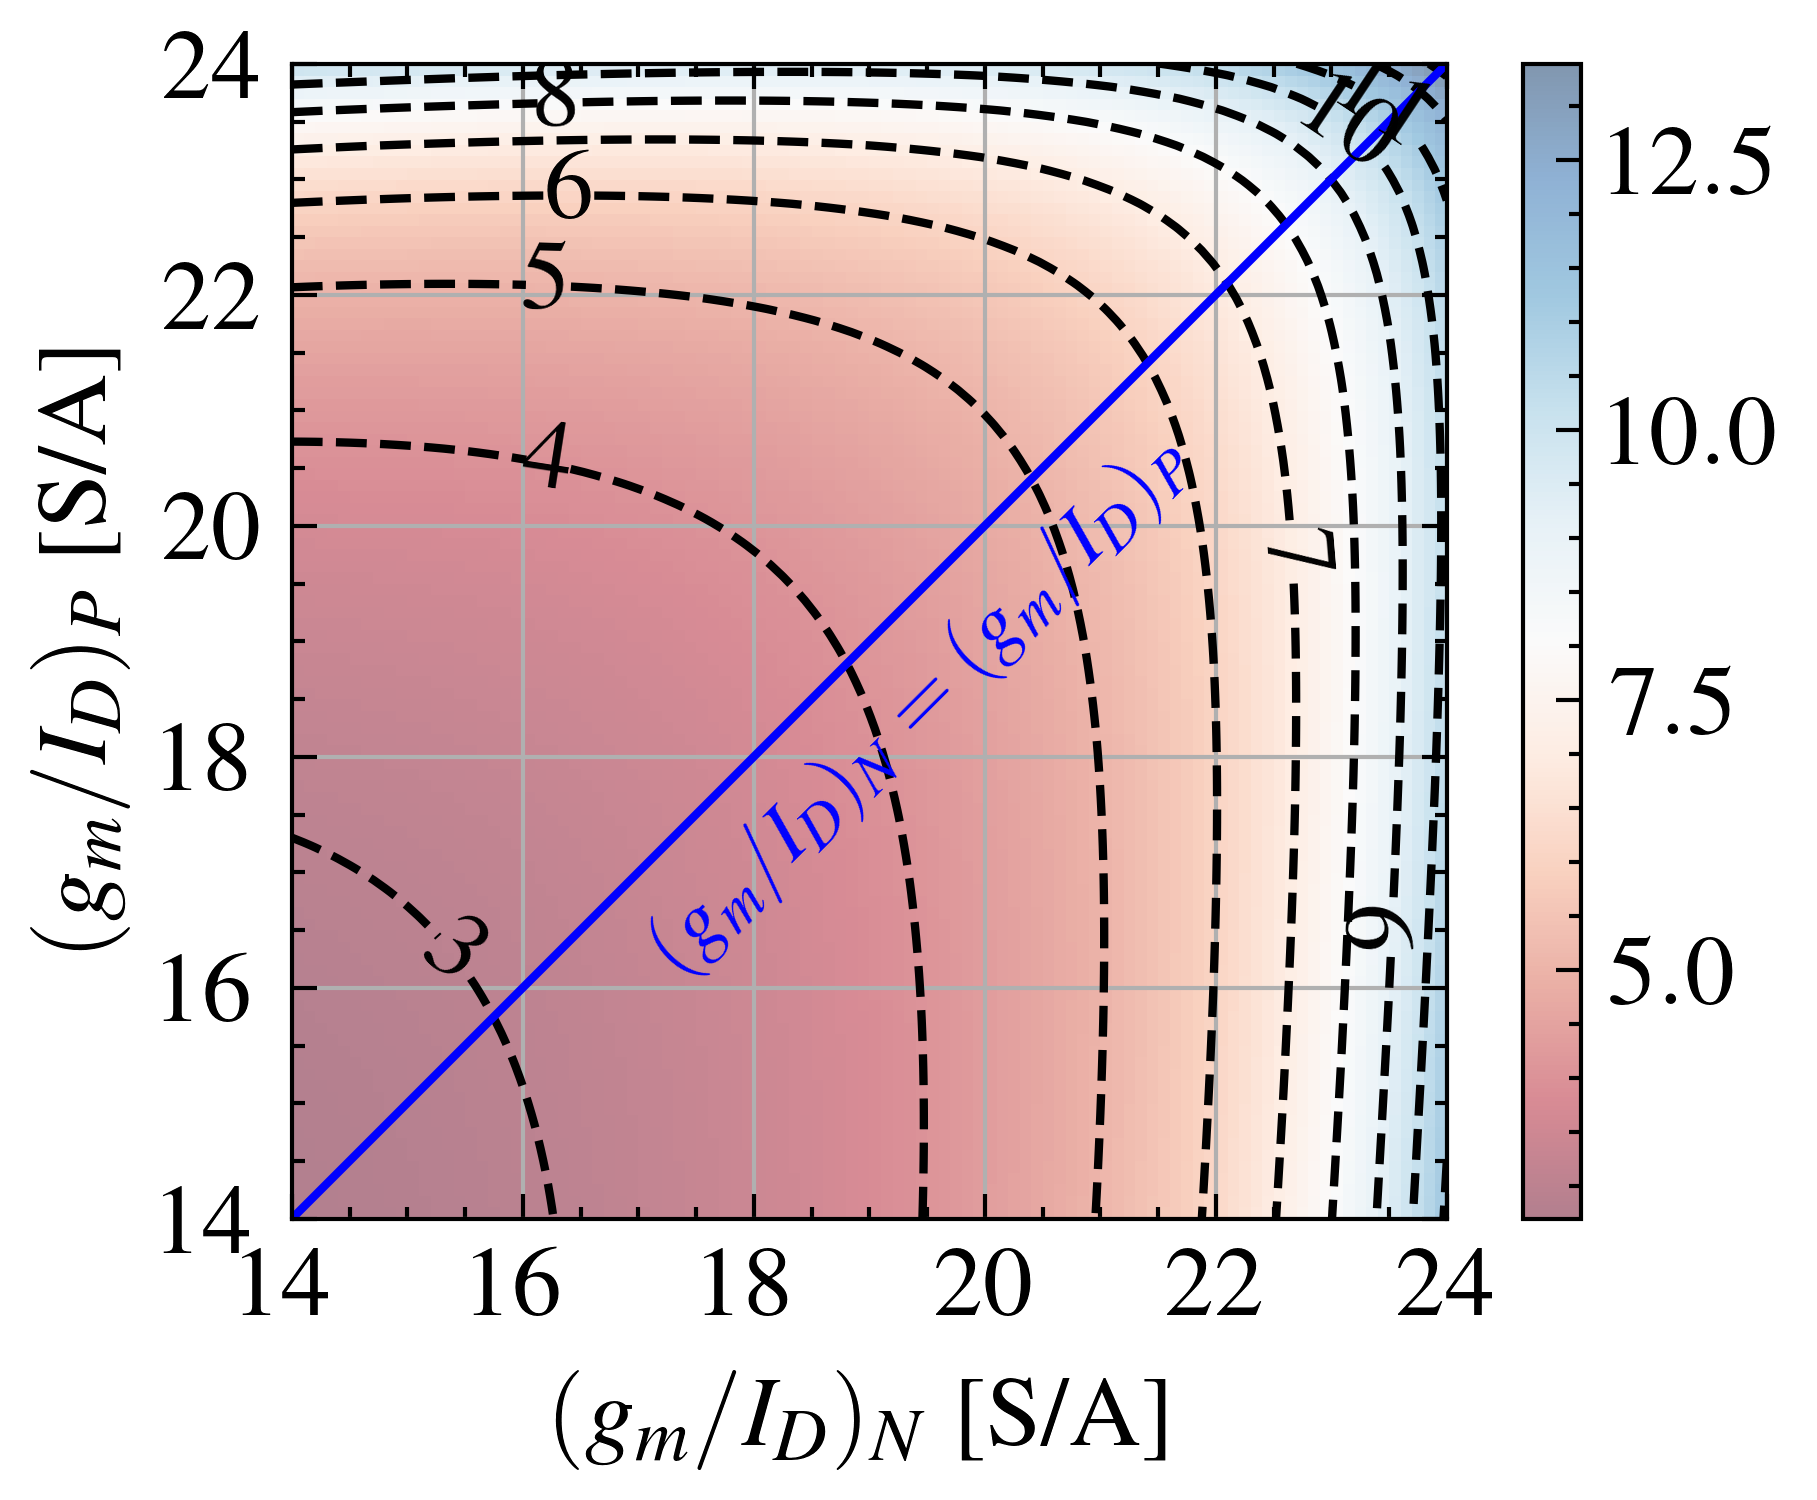
\includegraphics[width=\linewidth]{img/CIN_CONTOUR.png}
            \caption[]%
            {{\small }}
            \label{fig:Cin Contour}
        \end{subfigure}
        \hfill
        \begin{subfigure}[c]{0.49\linewidth}  
            \centering 
            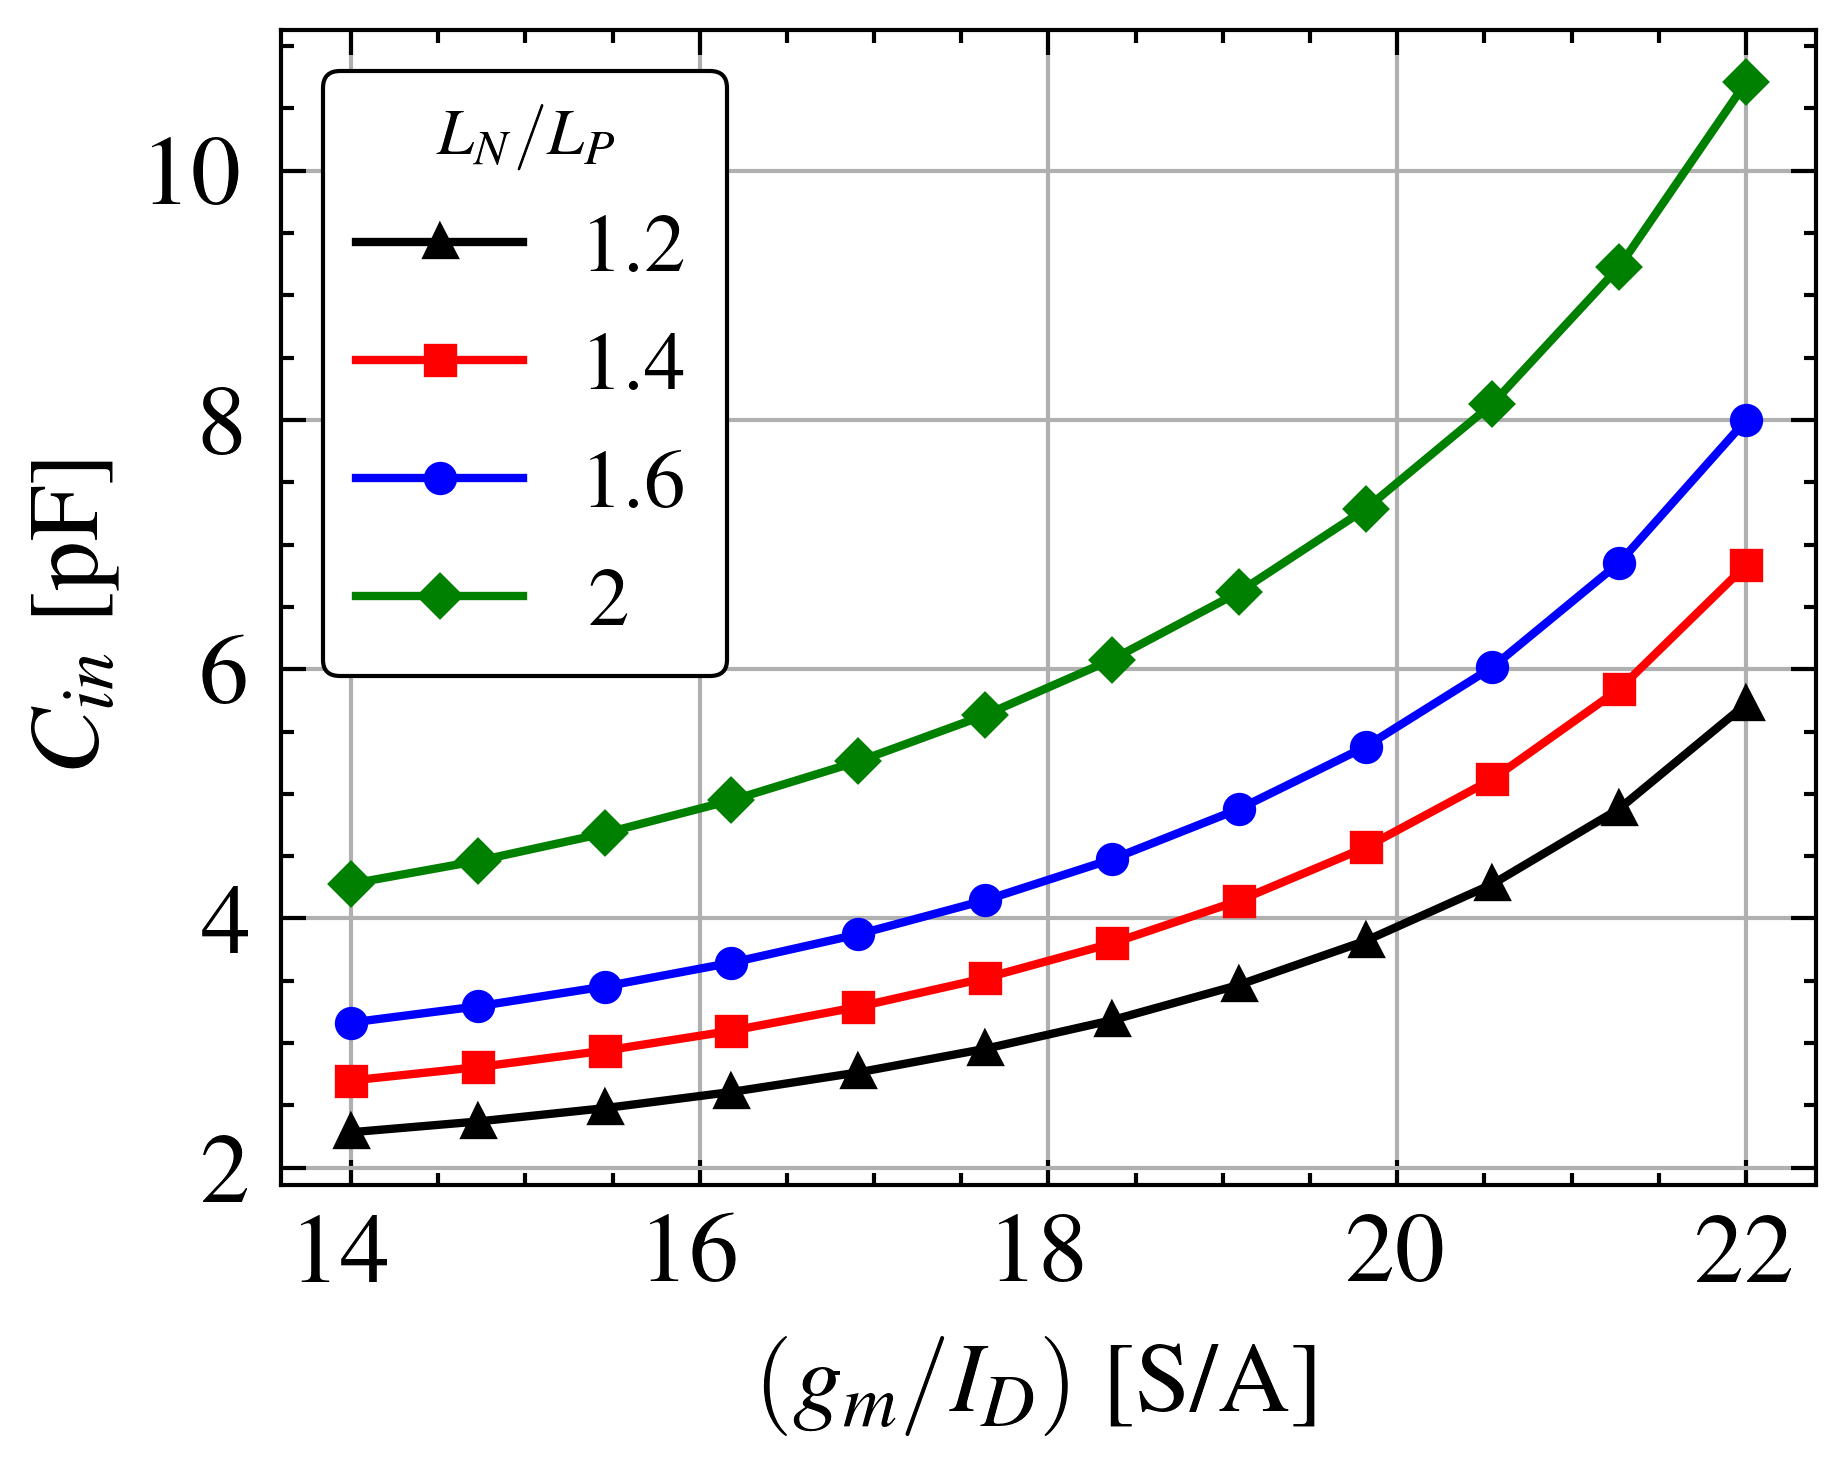
\includegraphics[width=\linewidth]{img/CIN-GMID.png}
            \caption[]%
            {{\small }}
            \label{fig:Cin Vs. GMID}
        \end{subfigure}
        \caption[ Don't write caption here ]
        {(a) $C_{in}$ [\si{\pico\farad}] as a  function of $(g_m/I_D)_N$ and $(g_m/I_D)_P$. (b) $C_{in}$ vs \gmID for various $L_N/L_P$ ($L_P=\SI{500}{\nano\metre}$), with IRN fixed at \SI{2}{\nano\volt\per\sqrt{\hertz}} } 
        \label{fig:Cin}
\end{figure}

\subsection{Area Constrained Applications} 
Bio-signal interfaces that capture many signals, particularly \textit{in vivo} brain signal monitoring, require low area AFEs \cite{yang2023ac}. Achieving channel areas below \SI{0.01}{\milli\metre^3} requires trading off area versus power efficiency. As shown in \cref{fig:Cin Contour} the proposed design methodology allows the input capacitance $C_{in}$ to be specified and the optimal \gmID to be selected to achieve the required thermal and flicker noise. \cref{fig:Cin Vs. GMID} shows the $C_{in}$ vs. \gmID requirement to meet the noise specification. In area constrained applications a smaller $C_{in}$ necessitates a lower \gmID. This, in turn, leads to an increased power requirement for the design.